\documentclass[12pt]{article}
\usepackage[table]{xcolor}
\usepackage[shortlabels]{enumitem}
\usepackage{tabularx,xltabular}
\usepackage{graphicx}
\usepackage{hyperref}
\usepackage{verbatim}
\usepackage{geometry}
\usepackage{ulem}
\usepackage[official]{eurosym}
\usepackage{tikz}
\usetikzlibrary{arrows,backgrounds,calc,decorations.markings,patterns,3d}
\usepackage{pgfplots}
\pgfplotsset{compat = newest}
\usetikzlibrary{fit}
\newcommand\addvmargin[1]{
\usetikzlibrary{arrows}
\node[fit=(current bounding box),inner ysep=#1,inner xsep=0]{};}
\usepackage{cancel}
\usepackage{fontspec}
\usepackage{array}  
\geometry{a4paper, top=2cm, left=2cm, right=2cm, bottom=2cm, headsep=1cm}
\usepackage{tabu}
\usepackage{pst-node}
\usepackage{colortbl}
\usepackage{array}
\usepackage{german}
\setlength\parindent{0pt}
\newcolumntype{?}{!{\vrule width 1pt}}
\usepackage{makecell}
\renewcommand{\arraystretch}{2.5}
\usepackage{pbox}
\usepackage{amssymb}
\usepackage{amsmath}
\usepackage{booktabs}
\newcolumntype{L}[1]{>{\raggedright\let\newline\\\arraybackslash\hspace{0pt}}m{#1}}
\newcolumntype{C}[1]{>{\centering\let\newline\\\arraybackslash\hspace{0pt}}m{#1}}
\newcolumntype{R}[1]{>{\raggedleft\let\newline\\\arraybackslash\hspace{0pt}}m{#1}}
\begin{document}
\rightline{Datum: 14.06.2023}
\centerline{{\Large Tägliche Übungen}} 
\vspace{1cm}
\noindent \\


\begin{xltabular}{\textwidth}{|C{0.75cm}|X|}
\arrayrulecolor{black}\hline
a)&$26=x+30$
\\\hline
b)&$42=y+6$
\\\hline
c)&$25=b-16$
\\\hline
d)&$5-b=19$
\\\hline
e)&$45-b=2$
\\\hline
f)&$38+a=39$
\\\hline
g)&$-29-4\cdot x+10\cdot x+13=8$
\\\hline
h)&$1\cdot x+4\cdot x-5-6=4$
\\\hline
i)&$13\cdot a-17-5\cdot a+2=81$
\\\hline
\end{xltabular}
\vspace{0.5cm}
\newpage
\rightline{Datum: 14.06.2023}
\centerline{{\large Lösungen Tägliche Übungen}} 
\vspace{0.5cm}

\begin{xltabular}{\textwidth}{|C{0.75cm}|X|}
\arrayrulecolor{black}\hline
a)&\begingroup\setlength{\jot}{-0.03cm}
\tikzstyle{background grid}=[draw, black!15,step=.5cm]
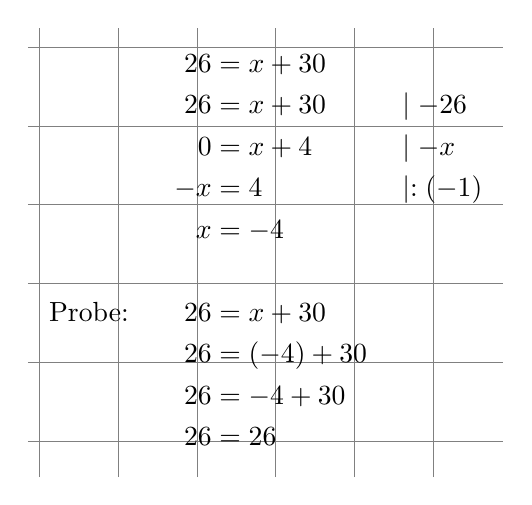
\begin{tikzpicture}[show background grid]
\node[below right] at (0,0.1) {
$\begin{aligned}
26 &=x+30& &  \\
26 &=x + 30& & \mid -26\\
0 &=x + 4& & \mid -x \\
-x &=4& & \mid :\left(-1\right)\\
x &=-4& & 
\\
\\
\mbox{Probe:}\qquad 26 &=x+30& &  \\
26 &=\left(-4\right)+30& &  \\
26 &=-4+30& &  \\
26 &=26& &  \\
\end{aligned}$};
\end{tikzpicture}
\endgroup
\\\hline
b)&\begingroup\setlength{\jot}{-0.03cm}
\tikzstyle{background grid}=[draw, black!15,step=.5cm]
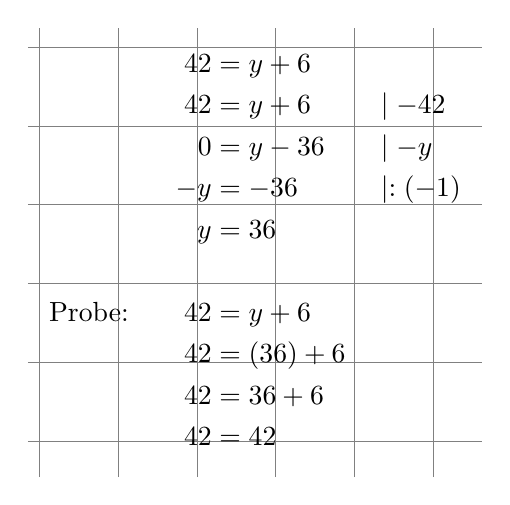
\begin{tikzpicture}[show background grid]
\node[below right] at (0,0.1) {
$\begin{aligned}
42 &=y+6& &  \\
42 &=y + 6& & \mid -42\\
0 &=y - 36& & \mid -y \\
-y &=-36& & \mid :\left(-1\right)\\
y &=36& & 
\\
\\
\mbox{Probe:}\qquad 42 &=y+6& &  \\
42 &=\left(36\right)+6& &  \\
42 &=36+6& &  \\
42 &=42& &  \\
\end{aligned}$};
\end{tikzpicture}
\endgroup
\\\hline
c)&\begingroup\setlength{\jot}{-0.03cm}
\tikzstyle{background grid}=[draw, black!15,step=.5cm]
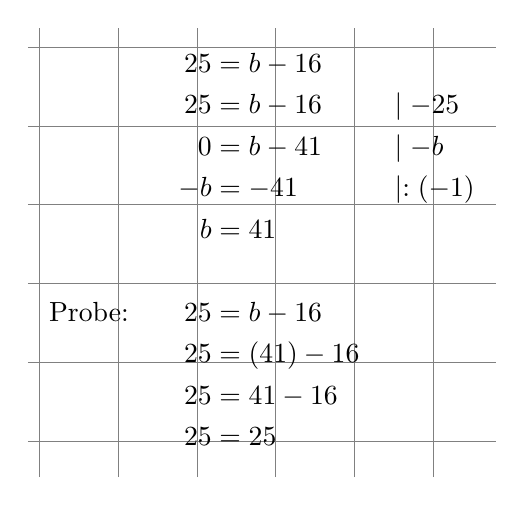
\begin{tikzpicture}[show background grid]
\node[below right] at (0,0.1) {
$\begin{aligned}
25 &=b-16& &  \\
25 &=b - 16& & \mid -25\\
0 &=b - 41& & \mid -b \\
-b &=-41& & \mid :\left(-1\right)\\
b &=41& & 
\\
\\
\mbox{Probe:}\qquad 25 &=b-16& &  \\
25 &=\left(41\right)-16& &  \\
25 &=41-16& &  \\
25 &=25& &  \\
\end{aligned}$};
\end{tikzpicture}
\endgroup
\\\hline
d)&\begingroup\setlength{\jot}{-0.03cm}
\tikzstyle{background grid}=[draw, black!15,step=.5cm]
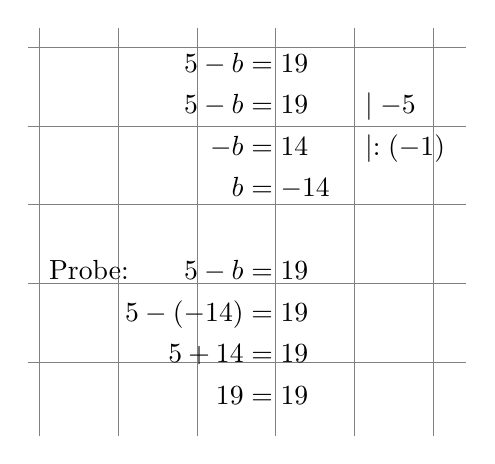
\begin{tikzpicture}[show background grid]
\node[below right] at (0,0.1) {
$\begin{aligned}
5-b &=19& &  \\
5 - b &=19& & \mid -5 \\
-b &=14& & \mid :\left(-1\right)\\
b &=-14& & 
\\
\\
\mbox{Probe:}\qquad 5-b &=19& &  \\
5-\left(-14\right) &=19& &  \\
5+14 &=19& &  \\
19 &=19& &  \\
\end{aligned}$};
\end{tikzpicture}
\endgroup
\\\hline
e)&\begingroup\setlength{\jot}{-0.03cm}
\tikzstyle{background grid}=[draw, black!15,step=.5cm]
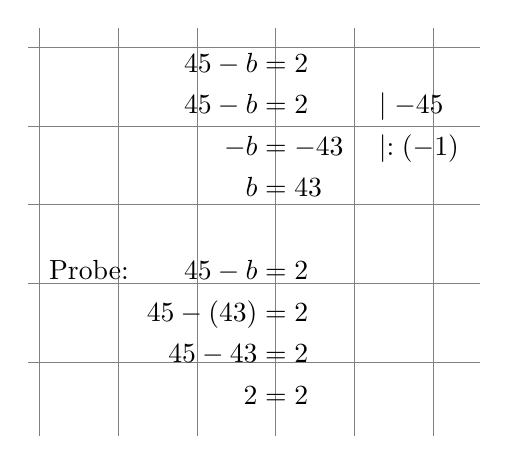
\begin{tikzpicture}[show background grid]
\node[below right] at (0,0.1) {
$\begin{aligned}
45-b &=2& &  \\
45 - b &=2& & \mid -45 \\
-b &=-43& & \mid :\left(-1\right)\\
b &=43& & 
\\
\\
\mbox{Probe:}\qquad 45-b &=2& &  \\
45-\left(43\right) &=2& &  \\
45-43 &=2& &  \\
2 &=2& &  \\
\end{aligned}$};
\end{tikzpicture}
\endgroup
\\\hline
f)&\begingroup\setlength{\jot}{-0.03cm}
\tikzstyle{background grid}=[draw, black!15,step=.5cm]
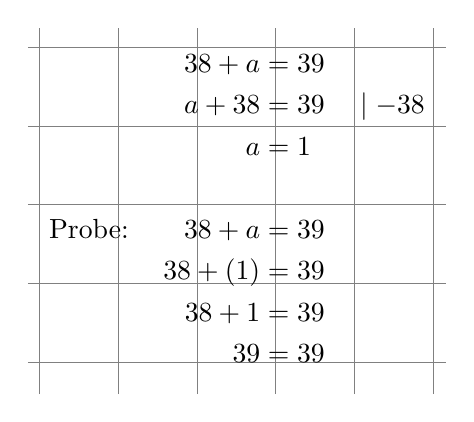
\begin{tikzpicture}[show background grid]
\node[below right] at (0,0.1) {
$\begin{aligned}
38+a &=39& &  \\
a + 38 &=39& & \mid - 38\\
a &=1& & 
\\
\\
\mbox{Probe:}\qquad 38+a &=39& &  \\
38+\left(1\right) &=39& &  \\
38+1 &=39& &  \\
39 &=39& &  \\
\end{aligned}$};
\end{tikzpicture}
\endgroup
\\\hline
g)&\begingroup\setlength{\jot}{-0.03cm}
\tikzstyle{background grid}=[draw, black!15,step=.5cm]
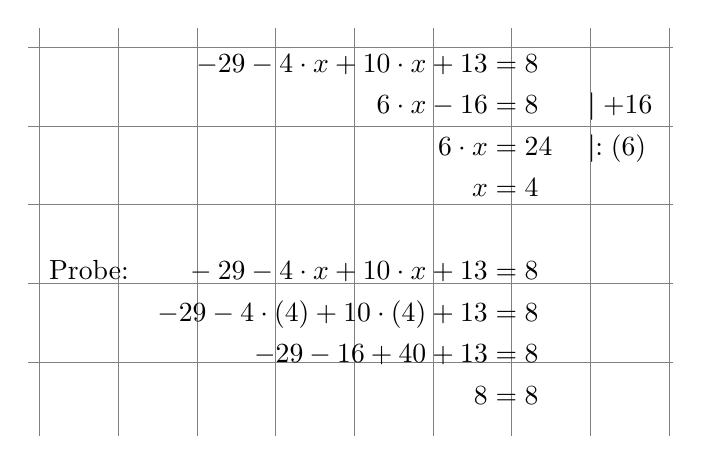
\begin{tikzpicture}[show background grid]
\node[below right] at (0,0.1) {
$\begin{aligned}
-29-4\cdot x+10\cdot x+13 &=8& &  \\
6\cdot x - 16 &=8& & \mid + 16\\
6\cdot x &=24& & \mid :\left(6\right)\\
x &=4& & 
\\
\\
\mbox{Probe:}\qquad -29-4\cdot x+10\cdot x+13 &=8& &  \\
-29-4\cdot \left(4\right)+10\cdot \left(4\right)+13 &=8& &  \\
-29-16+40+13 &=8& &  \\
8 &=8& &  \\
\end{aligned}$};
\end{tikzpicture}
\endgroup
\\\hline
h)&\begingroup\setlength{\jot}{-0.03cm}
\tikzstyle{background grid}=[draw, black!15,step=.5cm]
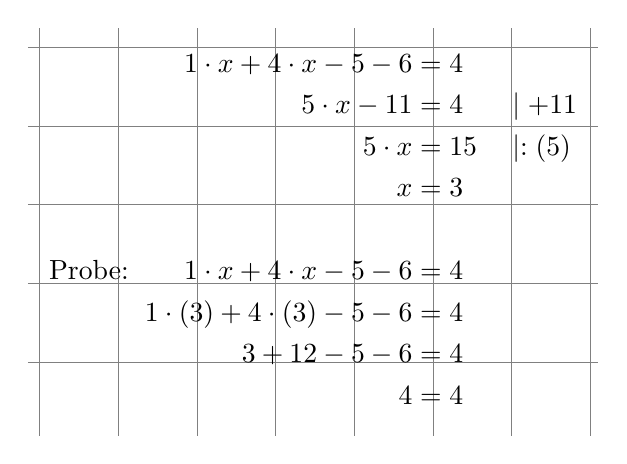
\begin{tikzpicture}[show background grid]
\node[below right] at (0,0.1) {
$\begin{aligned}
1\cdot x+4\cdot x-5-6 &=4& &  \\
5\cdot x - 11 &=4& & \mid + 11\\
5\cdot x &=15& & \mid :\left(5\right)\\
x &=3& & 
\\
\\
\mbox{Probe:}\qquad 1\cdot x+4\cdot x-5-6 &=4& &  \\
1\cdot \left(3\right)+4\cdot \left(3\right)-5-6 &=4& &  \\
3+12-5-6 &=4& &  \\
4 &=4& &  \\
\end{aligned}$};
\end{tikzpicture}
\endgroup
\\\hline
i)&\begingroup\setlength{\jot}{-0.03cm}
\tikzstyle{background grid}=[draw, black!15,step=.5cm]
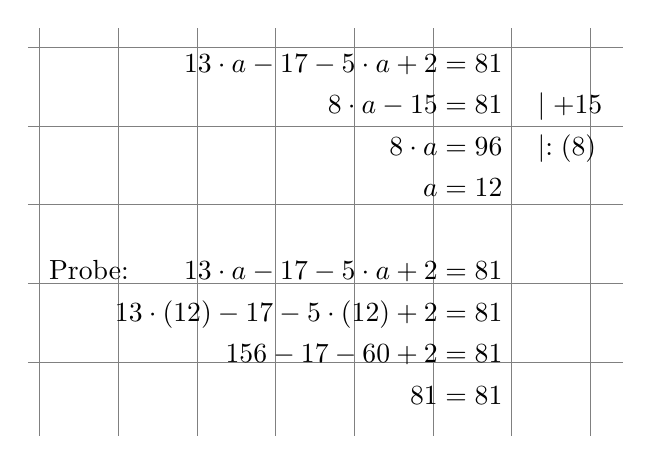
\begin{tikzpicture}[show background grid]
\node[below right] at (0,0.1) {
$\begin{aligned}
13\cdot a-17-5\cdot a+2 &=81& &  \\
8\cdot a - 15 &=81& & \mid + 15\\
8\cdot a &=96& & \mid :\left(8\right)\\
a &=12& & 
\\
\\
\mbox{Probe:}\qquad 13\cdot a-17-5\cdot a+2 &=81& &  \\
13\cdot \left(12\right)-17-5\cdot \left(12\right)+2 &=81& &  \\
156-17-60+2 &=81& &  \\
81 &=81& &  \\
\end{aligned}$};
\end{tikzpicture}
\endgroup
\\\hline
\end{xltabular}
\vspace{0.5cm}
\end{document}